\documentclass{standalone}
\usepackage[T1]{fontenc}
\usepackage[utf8]{inputenc}
\usepackage{pgf,tikz}
\usepackage{pgfplots}
\RequirePackage[amssymb]{SIunits}
%\pgfplotsset{compat=1.9}


\begin{document}


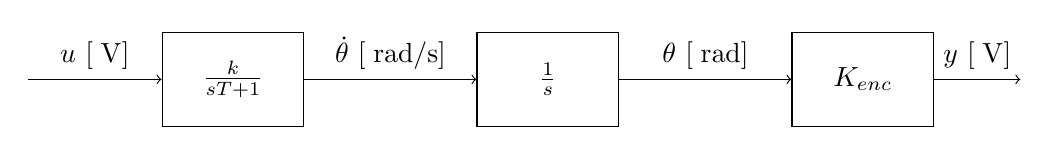
\begin{tikzpicture}[
    node distance=3cm, block/.style={rectangle, draw, minimum height=12mm, minimum width=18mm}, sumnode/.style={circle, draw, inner sep=1pt}]

  \node[coordinate] (input) {};
  \node[block, right of=input, node distance=26mm] (DC) {$\frac{k}{sT+1}$};
  \node[block, right of=DC, node distance=40mm] (int) {$\frac{1}{s}$};
  \node[block,right of=int, node distance=40mm] (enc) {$K_{enc}$};
  \node[coordinate, right of=enc, node distance=20mm] (output) {};

  \draw[->] (input) -- node[above] {$u$ [\unit{}{\volt}]} (DC);
  \draw[->] (DC) -- node[above] {$\dot{\theta}$ [\unit{}{\rad\per\second}]} (int);
  \draw[->] (int) -- node[above] {$\theta$ [\unit{}{\rad}]} (enc);
  \draw[->] (enc) -- node[above] {$y$ [\unit{}{\volt}]} (output);

\end{tikzpicture}
\end{document}


